%! Author = mariuszindel
%! Date = 25.01.21

\section{Modulationen}

\subsection{Amplitudenmodulation}
\begin{center}
    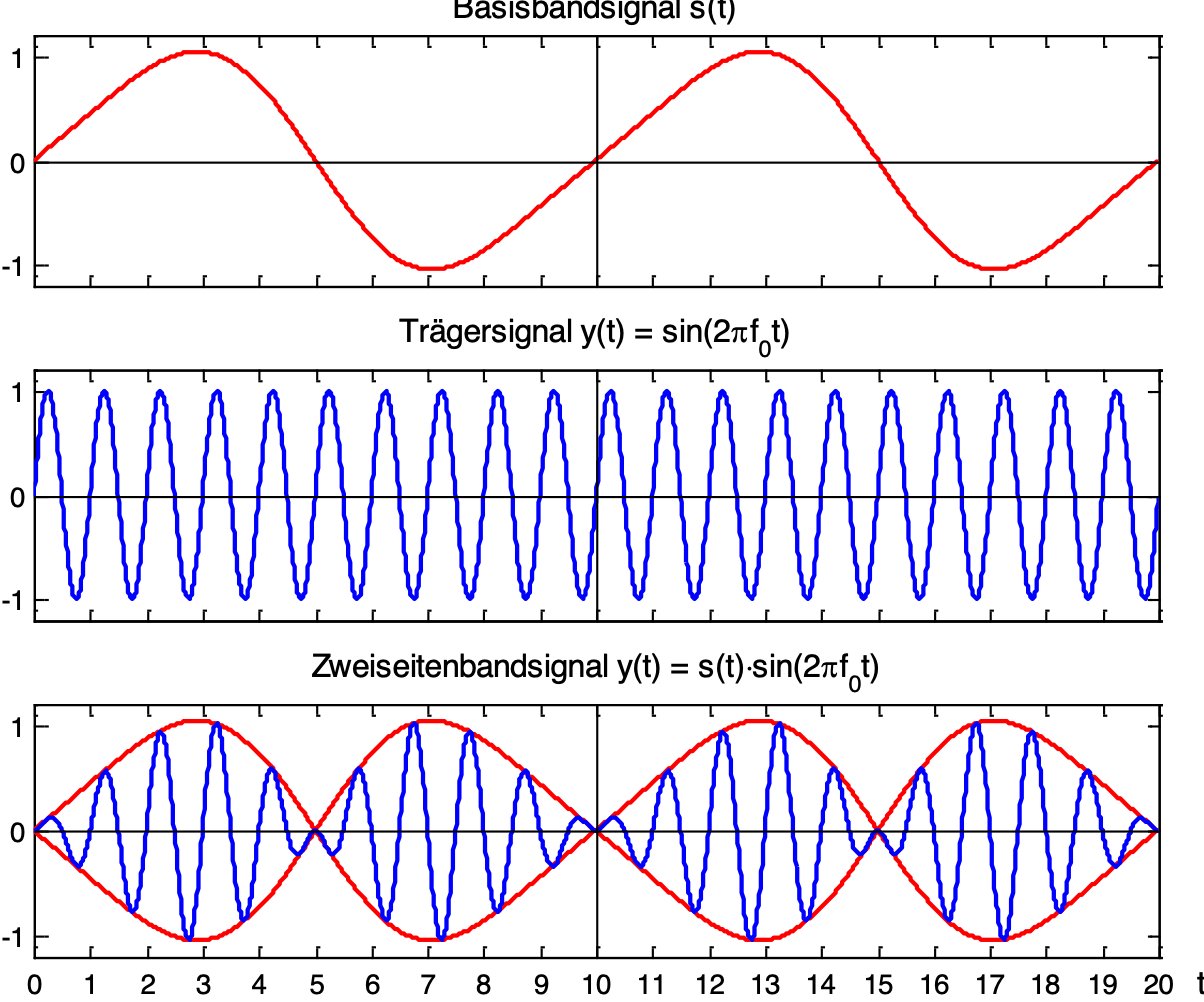
\includegraphics[width=\linewidth]{graphic/fourier/Amplitudenmodulation.png}
\end{center}
\vspace{-8pt}

\subsubsection{Oberes und Unteres Seitenband}
\begin{center}
    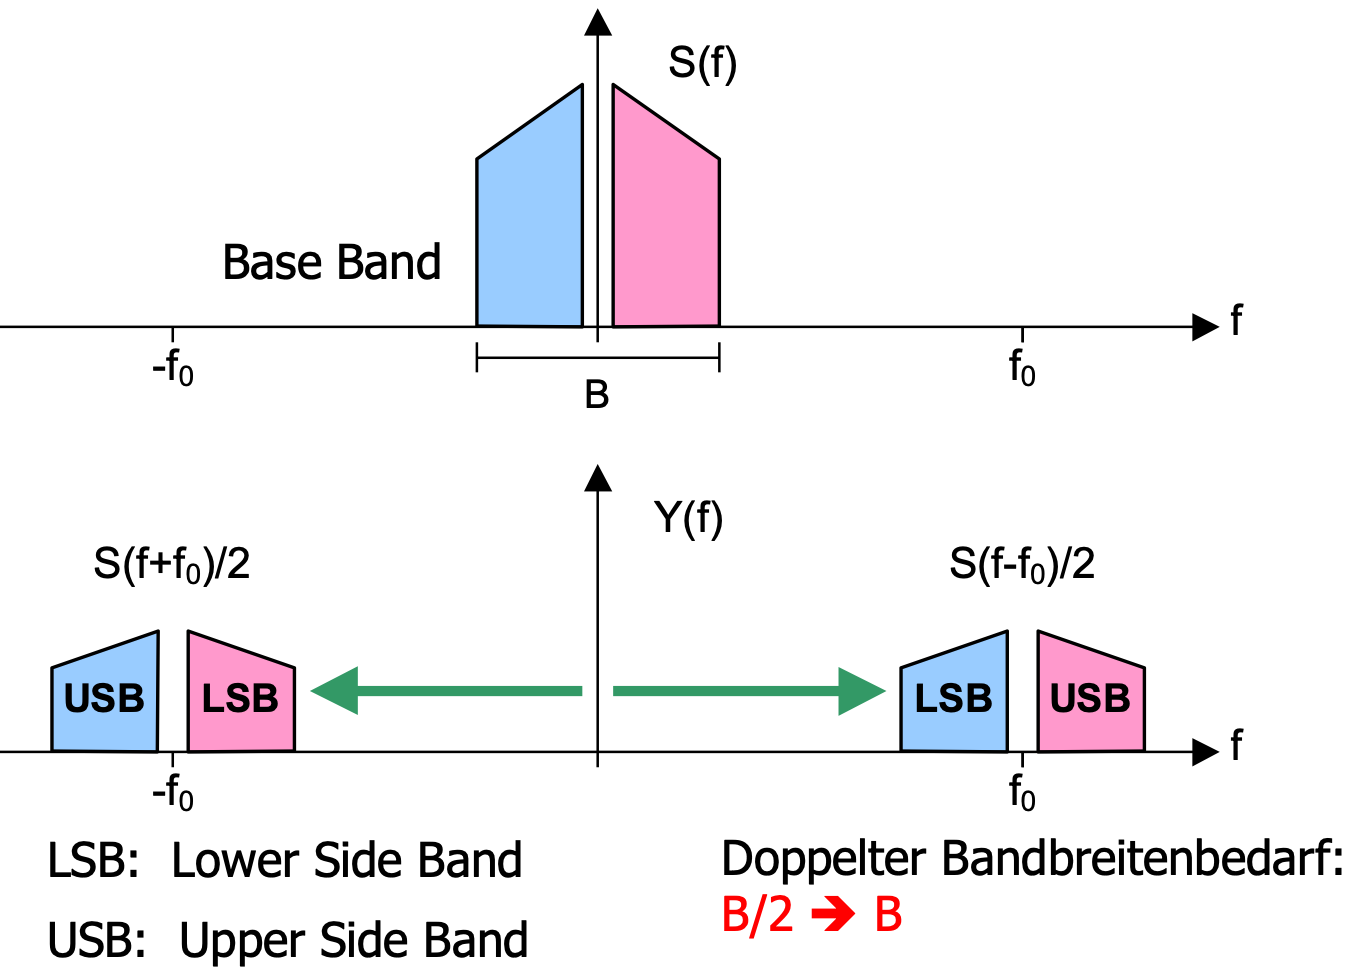
\includegraphics[width=\linewidth]{graphic/fourier/Oberes und Unteres Seitenband.png}
\end{center}
\vspace{-8pt}

\subsection{Tonhöhenverschiebung}
\subsubsection{Lösung 1:}
\begin{itemize}
    \item Elimination des oberen Seitenbandes (USB) durch ein Tiefpassfilter mit der Grendfrequenz (diese auslesen was muss wohin geschoben werden)
    \item Demodulation mit einer LO-Frequenz von X (Auslesen), welches das untere Seitenband (LSB) mit einem Frequenzshift von X in das Basisband zurückschiebt
\end{itemize}
\subsubsection{Lösung 2:}
\begin{itemize}
    \item Elimination des unteren Seitenbandes (LSB) durch ein Hochpassfilter mit der Grenzfre- quenz X (auslesen)
    \item Demodulation mit einer LO-Frequenz von X (auslesen), welches das obere Seitenband (USB) mit einem Frequenzshift von X in das Basisband zurückschiebt.
\end{itemize}
\subsubsection{Massnahmen nach der Verschiebung:}
\begin{itemize}
    \item Durch die Demodulation ensteht eine Spektrumskomponente bei der doppelten Trägerfre- quenz von ca. 16kHz
    \item Die hörbaren Frequenzanteile können mit einem Tiefpassfilter eliminiert werden.
\end{itemize}

\subsection{Digitale Modulationsverfahren}
\subsubsection{Amplitudenumtastung (ASK)}
\begin{center}
    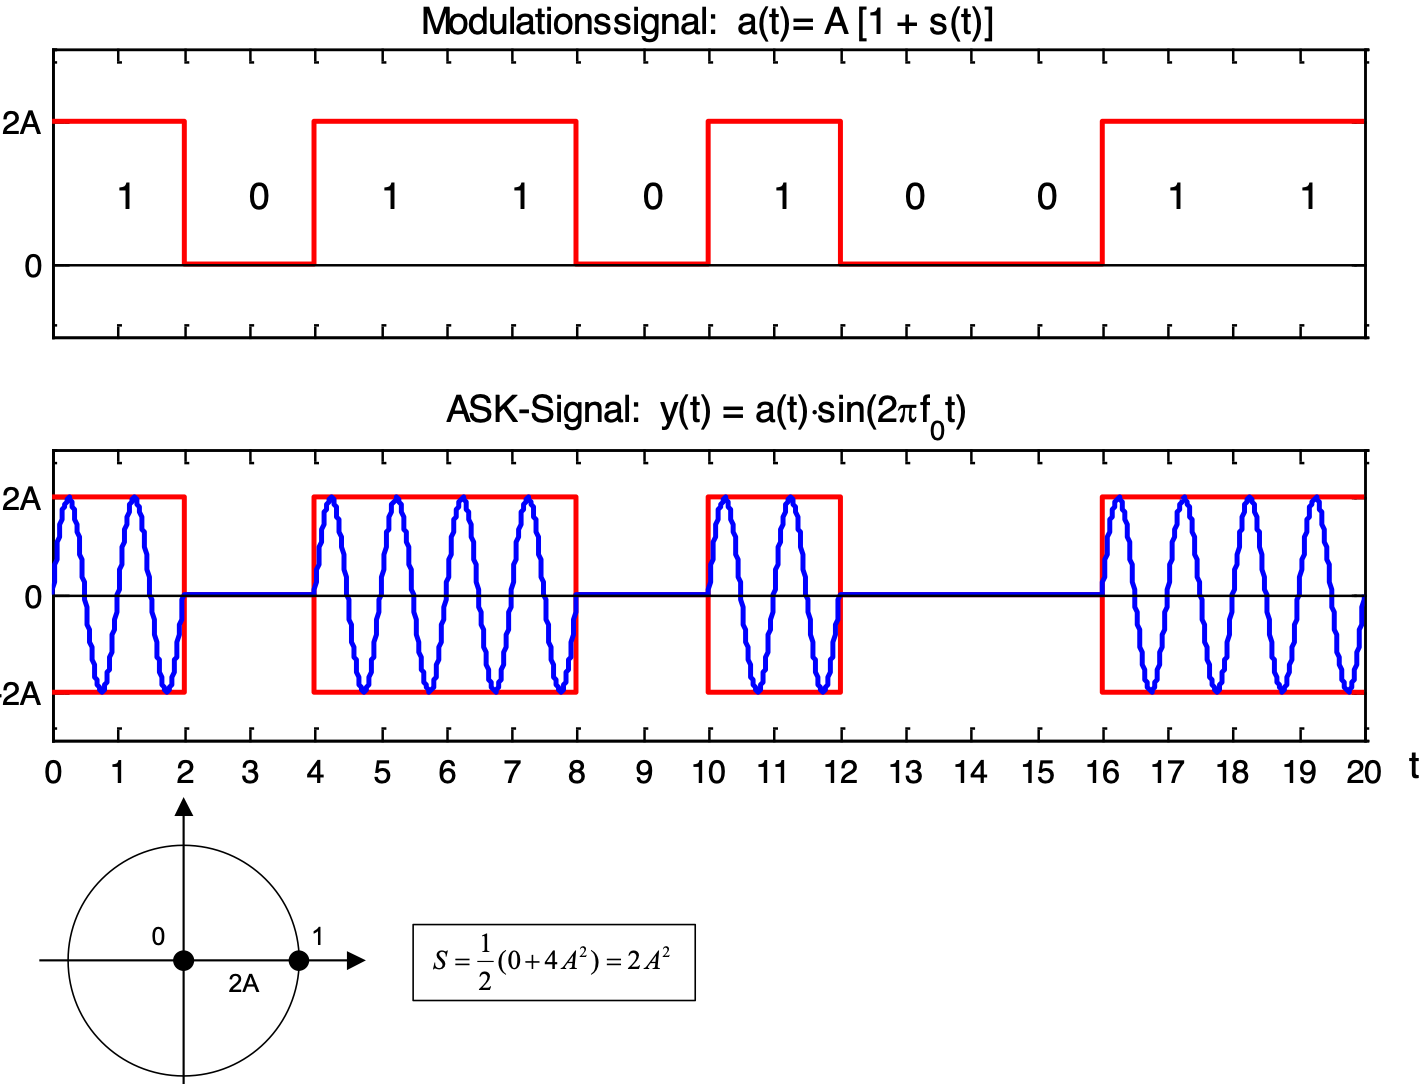
\includegraphics[width=\linewidth]{graphic/fourier/Amplitudenumtastung.png}
\end{center}
\vspace{-8pt}

\subsubsection{Phasenumtastung (PSK)}
\begin{center}
    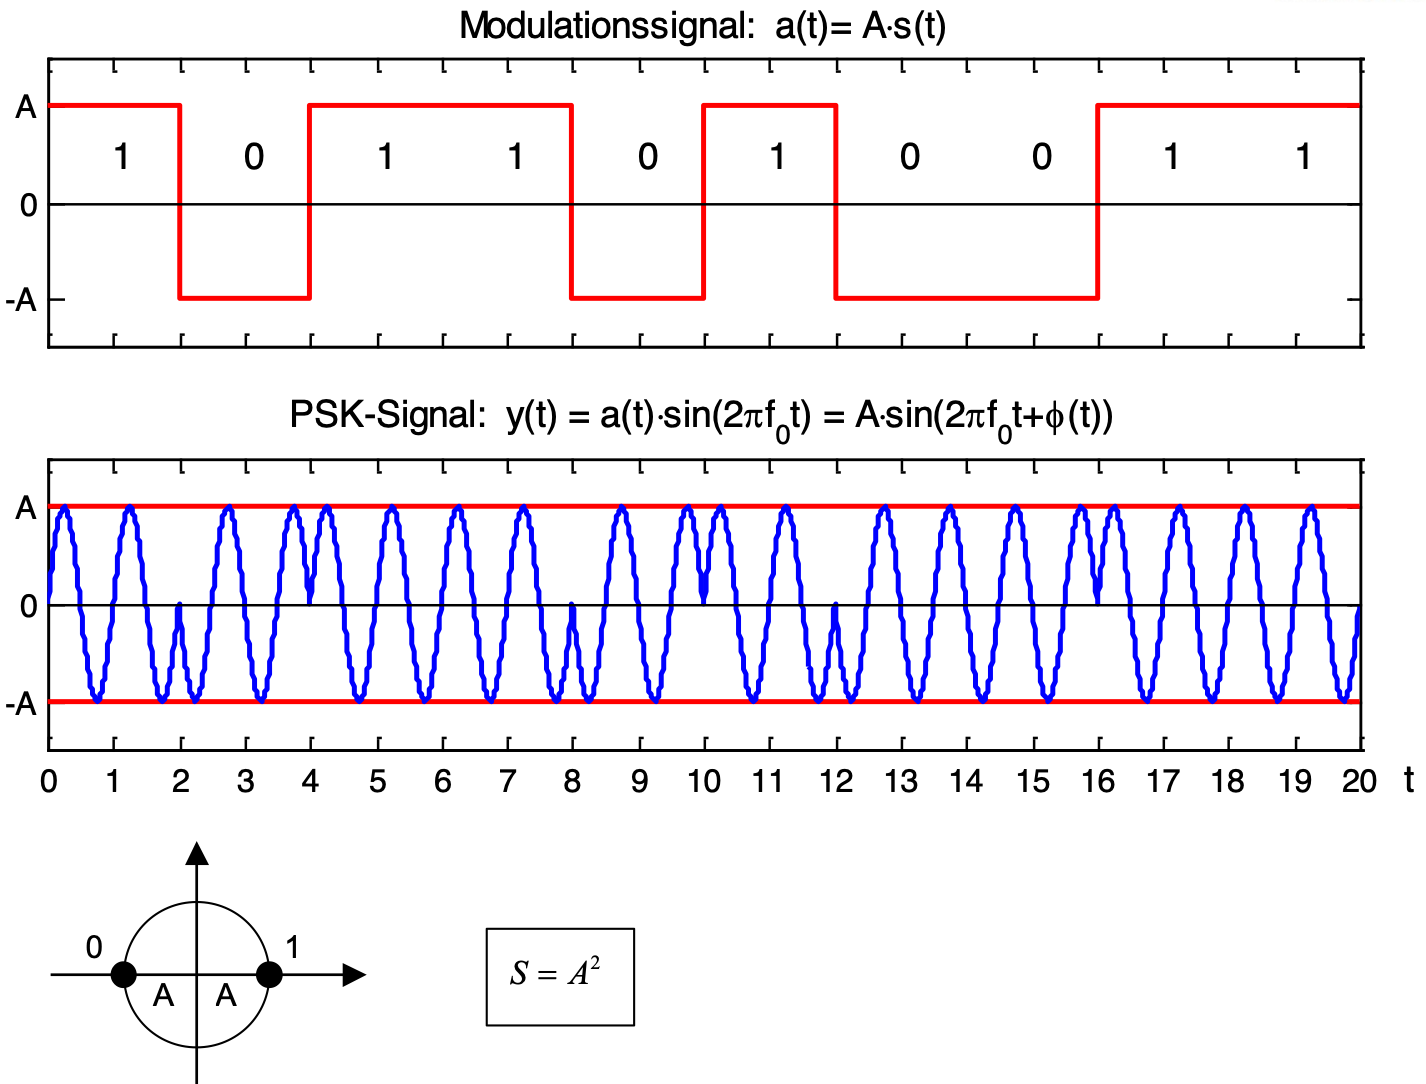
\includegraphics[width=\linewidth]{graphic/fourier/Phasenumtastung.png}
\end{center}
\vspace{-8pt}

\subsubsection{Differentielle Phasenumtastung (DPSK)}
\begin{center}
    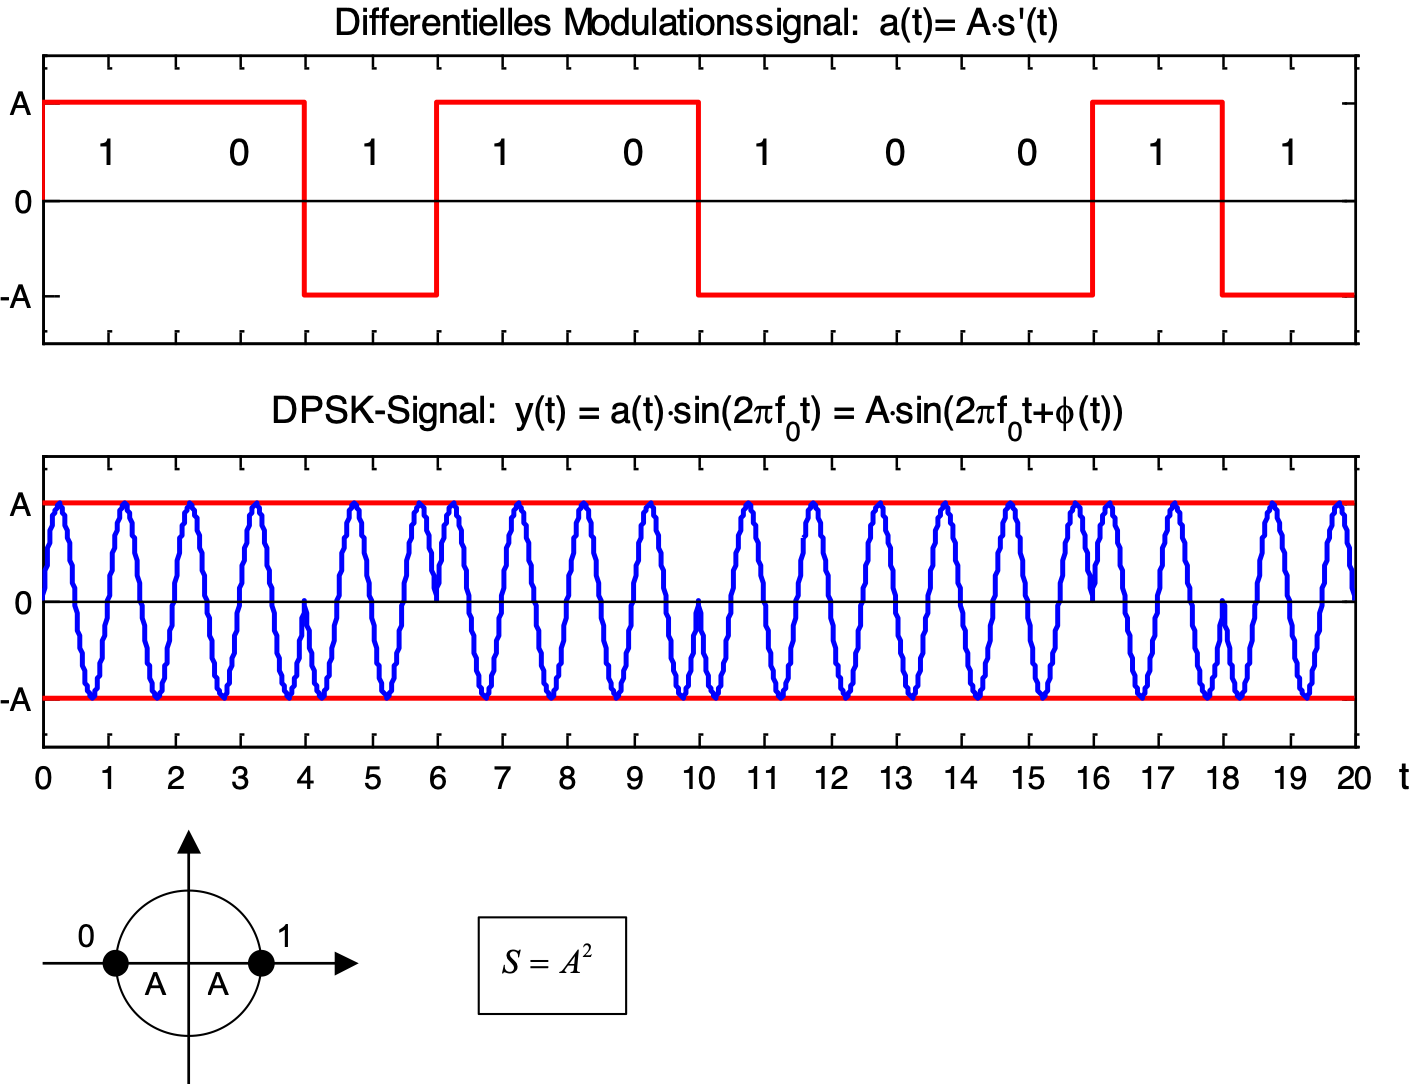
\includegraphics[width=\linewidth]{graphic/fourier/Differentielle Phasenumtastung.png}
\end{center}
\vspace{-8pt}

\subsubsection{Mehrstufige Amplitudenumtastung (PAM)}
\begin{center}
    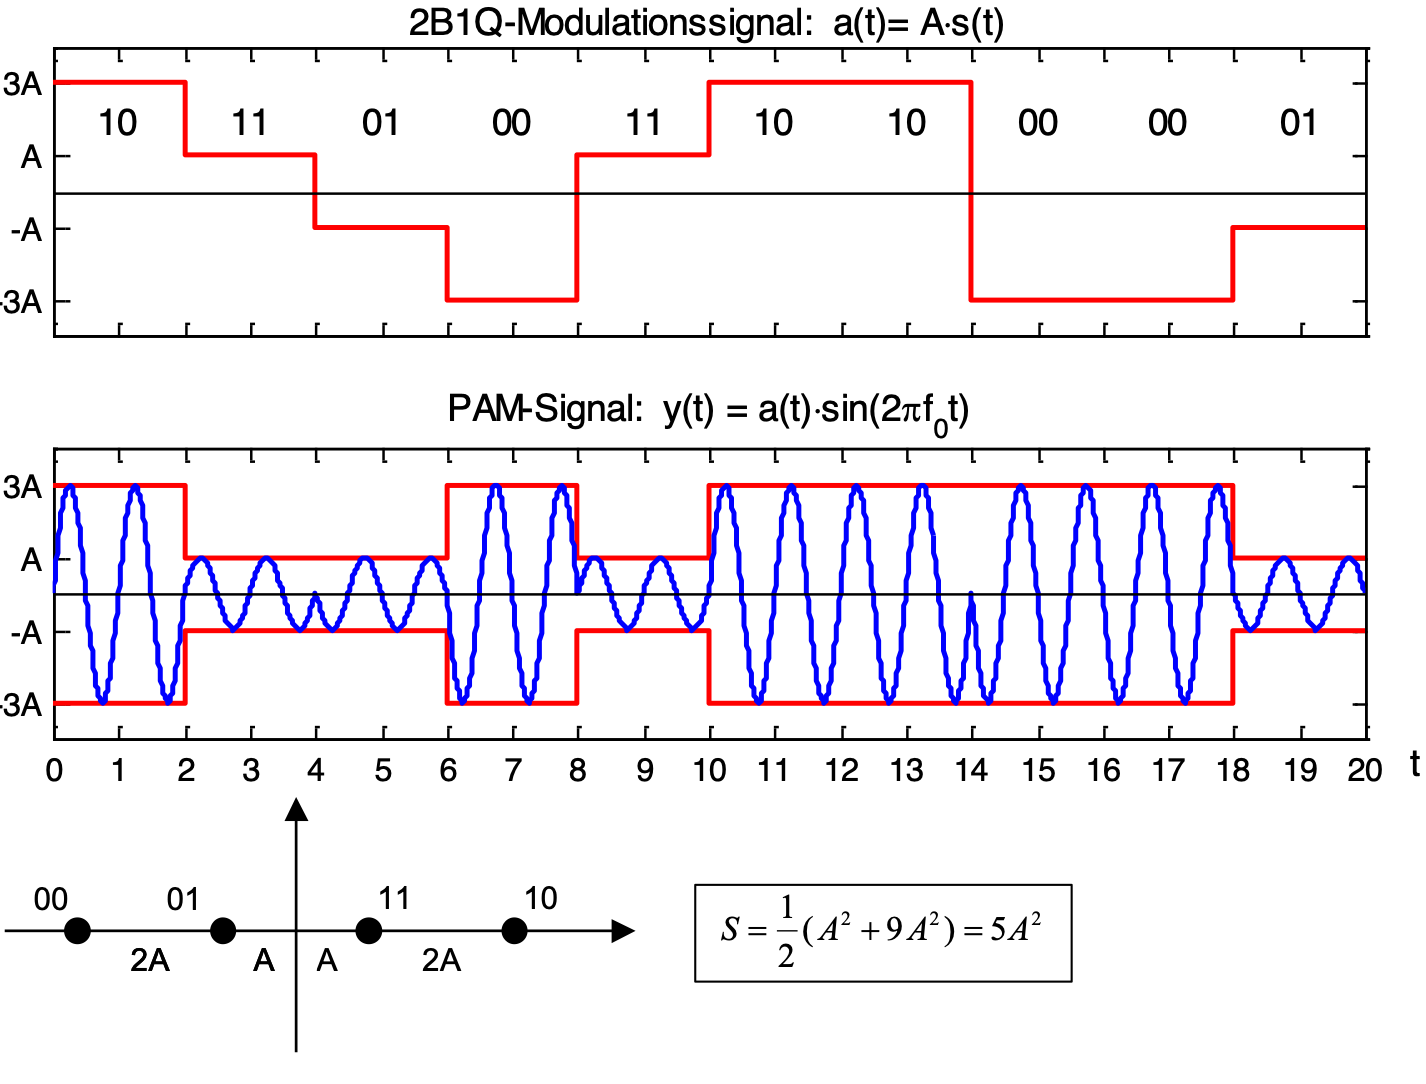
\includegraphics[width=\linewidth]{graphic/fourier/Mehrstufige Amplitudenumtastung.png}
\end{center}
\vspace{-8pt}

\subsubsection{Mehrstufige Phasenumtastung (QPSK)}
\begin{center}
    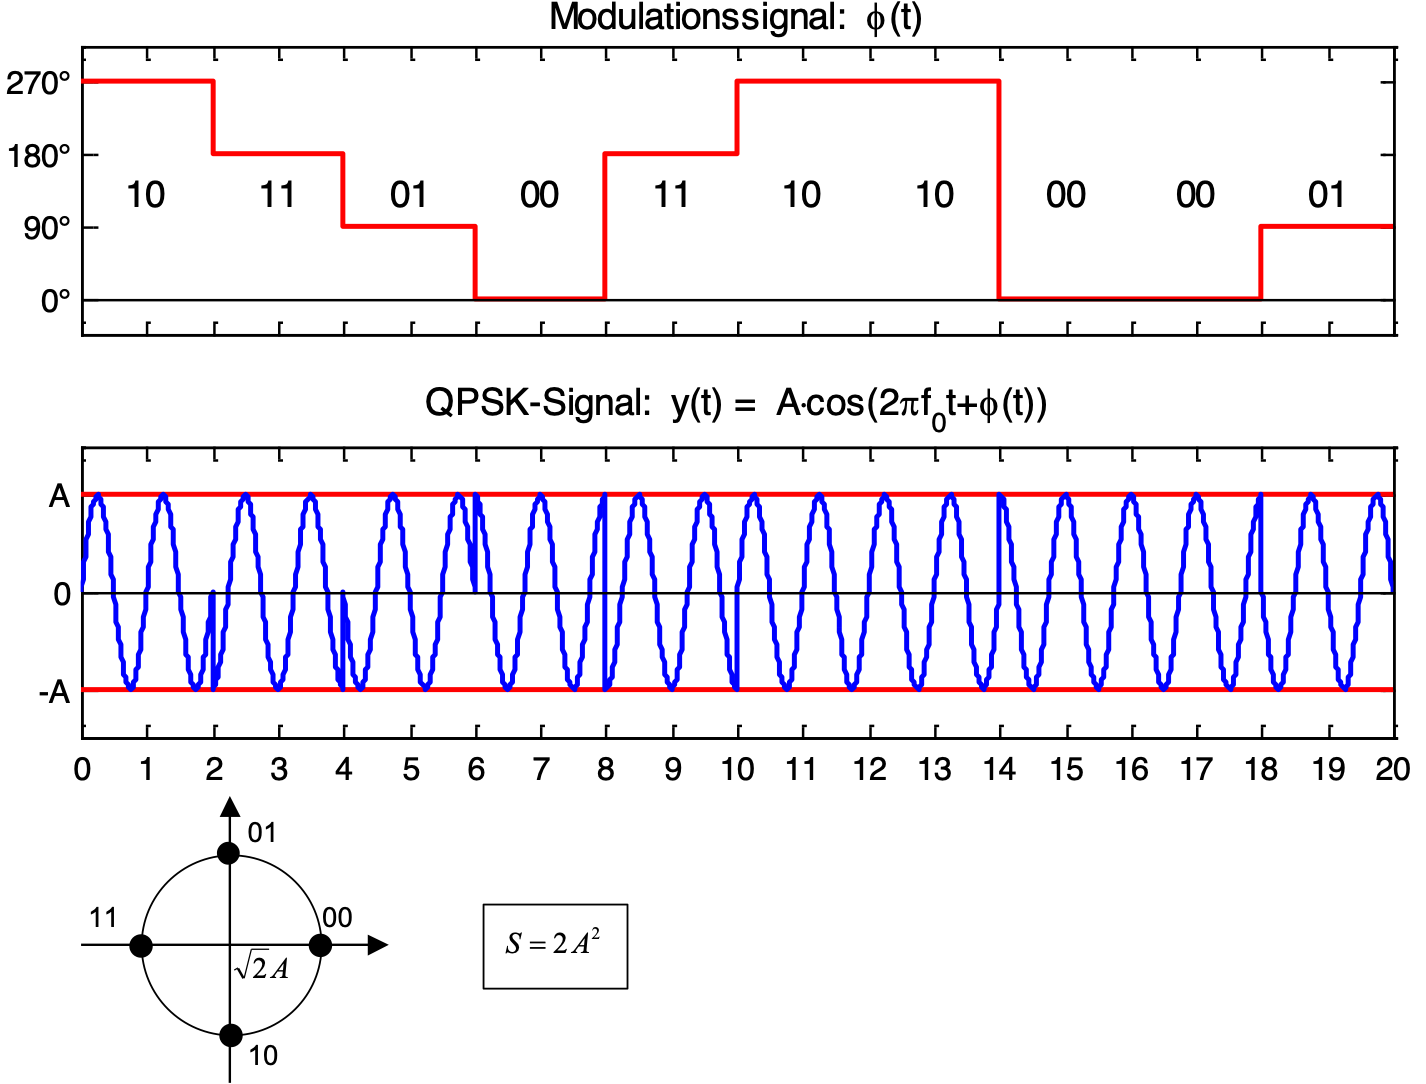
\includegraphics[width=\linewidth]{graphic/fourier/Mehrstufige Phasenumtastung.png}
\end{center}
\vspace{-8pt}


\subsubsection{QAM}
\begin{center}
    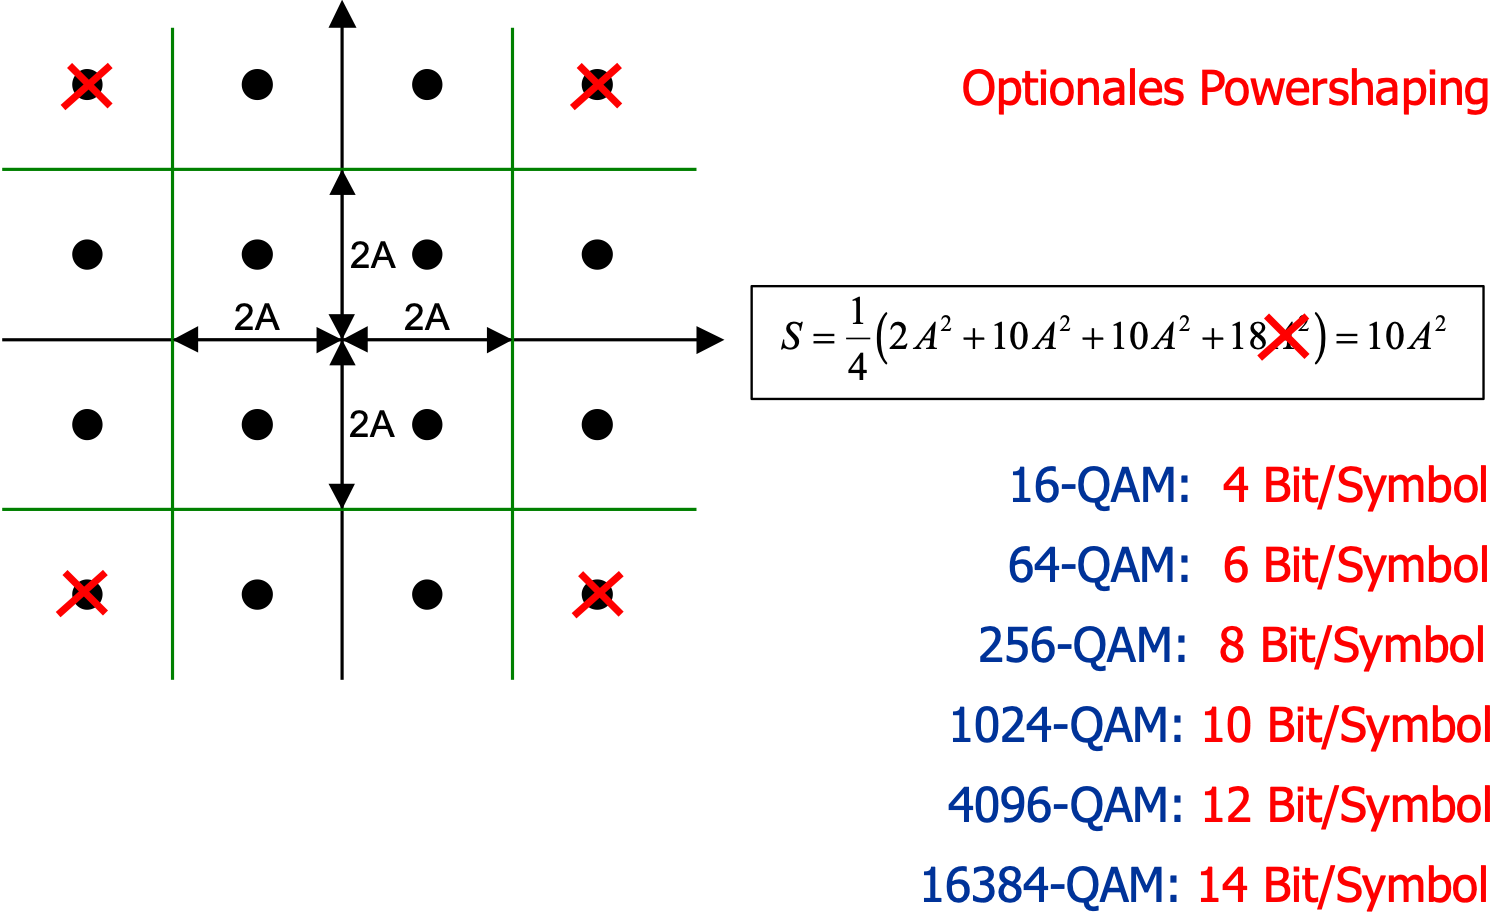
\includegraphics[width=\linewidth]{graphic/fourier/QAM.png}
\end{center}
\vspace{-8pt}
